\documentclass{article}

\usepackage[a4paper, margin=1in, includefoot]{geometry}
\usepackage[subsectionbib]{bibunits}

\usepackage{xcolor}
\usepackage{amssymb}
\usepackage{xcolor}
\usepackage{mathtools}

\usepackage{cite}
\usepackage{amsmath,amssymb,amsfonts}
\usepackage{algorithmic}
\usepackage{graphicx}
\usepackage{textcomp}

\usepackage{cancel}

\usepackage{multirow}

\usepackage{bm} 
\usepackage{pifont}
\usepackage{tikz}
\usetikzlibrary{automata}
%\usetikzlibrary{standalone}
\usetikzlibrary{shapes,arrows}
\newcommand{\cmark}{\ding{51}}%
\newcommand{\xmark}{\ding{55}}%
% \usepackage{cancel}
% \usepackage{tikz}
% \usetikzlibrary{automata}
% \usetikzlibrary{shapes,arrows}
% \usepackage{booktabs}
% \usepackage{url}
\usepackage{hyperref}

\newtheorem{ass}{\it{Assumption}}
\newtheorem{mydef}{\it{Definition}}
\newtheorem{lem}{\it{Lemma}}
\newtheorem{myeg}{\it{Example}}
\newtheorem{thm}{\it{Theorem}}
%\newtheorem{proof}{\it{Proof}}
\newtheorem{mycomp}{{\color{magenta}{\it{\bf My computations}}}}
\newtheorem{prop}{\it{Proposition}}
\newtheorem{assum}{\it{Assumption}}
\newtheorem{cor}{\it{Corollary}}
\newtheorem{rem}{\it{Remark}}
\newtheorem{pb}{\it{Problem}}
\newtheorem{cl}{\it{Claim}}
\usepackage{hyperref}

\makeatletter
%%%%%%%%%%%%%%%%%%%%%%%%%%%%%%%%%%%%%%%%%%%%%%%%%%%%%%%%%%%%%%%%%%%%%%%%%%%%%%%%
%%%%% Due to the usage of mathbbol we need to redefine \!
%%%%%%%%%%%%%%%%%%%%%%%%%%%%%%%%%%%%%%%%%%%%%%%%%%%%%%%%%%%%%%%%%%%%%%%%%%%%%%%%
\renewcommand{\!}{\tmspace-\thinmuskip{.1667em}}
%%%%%%%%%%%%%%%%%%%%%%%%%%%%%%%%%%%%%%%%%%%%%%%%%%%%%%%%%%%%%%%%%%%%%%%%%%%%%%%%
%%%%% For the references above equality and others relationships in equations
%%%%%%%%%%%%%%%%%%%%%%%%%%%%%%%%%%%%%%%%%%%%%%%%%%%%%%%%%%%%%%%%%%%%%%%%%%%%%%%%
\newcounter{relctr} %% <- counter for relations
\everydisplay\expandafter{\the\everydisplay\setcounter{relctr}{0}} %% <- reset every eq
\renewcommand*\therelctr{\alph{relctr}} %% <- label format
%%%%%%%%%%%%%%%%%%%%%%%%%%%%%%%%%%%%%%%%%%%%%%%%%%%%%%%%%%%%%%%%%%%%%%%%%%%%%%%%
\newcommand\labelrel[2]{%
  \begingroup
    \refstepcounter{relctr}%
    \stackrel{\textnormal{(\alph{relctr})}}{\mathstrut{#1}}%
    \originallabel{#2}%
  \endgroup
}
\AtBeginDocument{\let\originallabel\label} %% <- store original definition
%%%%%%%%%%%%%%%%%%%%%%%%%%%%%%%%%%%%%%%%%%%%%%%%%%%%%%%%%%%%%%%%%%%%%%%%%%%%%%%%
\makeatother

\counterwithin*{figure}{section}

\title{\textbf{Statement of Changes --- Authors' response}}
\author{Y. \textbf{Zacchia Lun}, F. \textbf{Santucci}, and A. \textbf{D'Innocenzo}}
\date{\vspace{-5ex}}
%\onehalfspacing
\begin{document}
\defaultbibliographystyle{IEEEtran} 
\defaultbibliography{biblio}
% \thispagestyle{empty}
% \hspace*{\fill} L'Aquila, {May 16, 2025}\\[1cm]
% Prof. Subhrakanti Dey\\
% Dept. of Electrical Engineering, Uppsala University\\\\
% \noindent
% Prof. Subhrakanti Dey,\\[2mm]
% \indent \textcolor{black}{Thank you for handling our manuscript ``Wireless Control With Channel State Detection And Message Dropout Compensation.'' We have carefully revised the manuscript and addressed all the issues.} For the reviewers' convenience, we have used blue-colored text in the revised version of the paper to highlight the main changes from the previous version.\\[2mm]
% \indent Our responses to the Associate Editor and Reviewers are in the following pages.\\[4mm]
% \noindent
% Sincerely,\\[4mm]
% \noindent
% Yuriy Zacchia Lun\\
% Fortunato Santucci\\
% Alessandro D'Innocenzo\\

% \clearpage
% \pagenumbering{arabic}
\maketitle
\tableofcontents
\vspace{2cm}
\noindent \textbf{Note:} The Associate Editor's and Reviewers' comments are typeset in \textit{italics} to enhance the clarity of this response letter, while our responses use the standard font. The excerpts of the manuscript reporting the main changes in the revised version are written in blue.

\section{Response to the Associate Editor}
\textbf{Associate Editor---General comment---}\textit{%
The paper was reviewed by three independent reviewers who all agree regarding the quality and relevance of the paper. }\\[2mm]
\textbf{Authors' response:} \textcolor{black}{We sincerely appreciate the constructive handling of the manuscript by the Associate Editor.}\\[4mm]
\textbf{Associate Editor---Comment 1---}\textit{%
Different technical comments should be addressed to further improve the paper. Please see the reviews for details.}\\[2mm]
\textbf{Authors' response:} \textcolor{black}{We thank the Associate Editor for gathering the valuable suggestions that enabled us to enhance the overall quality of the manuscript. In the revised version, we have addressed all the Reviewers' concerns and implemented the necessary modifications.}
\section{Response to Reviewer 9}
% \begin{bibunit}
\textbf{Reviewer 9—General comments—}\textit{%
This letter discusses an interesting topic about the number of future control inputs to transfer in the wireless networked control systems. However, this version is a little mess in notations, descriptions, resulting a challenge of readability. I believe a major improvement is necessary for publishing. The comments are as follows.}\\[2mm]
\textbf{Authors' response:} \textcolor{black}{We appreciate the Reviewer's feedback. In the revised version, we have carefully addressed the Reviewer's concerns and made necessary modifications.}\\[4mm]
%%%
\textbf{Reviewer 9–Comment 1—}\textit{%
Motivation is not enough, especially in the Sec. I—Introduction, it is not clearly for the contribution through comparing with the existing relevant research. 
Besides, authors underline that a practical hidden Markov jump linear system (HMJLS) model is one of the contributions of this letter. 
I wonder if it is the first time to propose it, or, you setup the model from a novel perspective. Description and analysis are necessary.}\\[2mm]
\textbf{Authors' response 1:} \textcolor{black}{We thank the Reviewer for the valuable comment. Due to the strict page limit of an L-CSS letter, we lack the space to provide an in-depth discussion of the state of the art, which is available in the references [1]–[5]. The relevance of the topic is thoroughly discussed there. This letter is motivated by two significant shortcomings of the previous relevant works, particularly [4] and [5]: the channel state information may be unavailable or imperfect, and transmitting future control inputs is a compelling alternative to sending only the current one, as outlined in the introduction. This letter addresses these two limitations of the previous research and significantly extends the results in [4]. The provided results greatly enhance the practical relevance of the wireless-channel-state-dependent control strategies by accounting for the channel state estimation with measurement noise and more advanced control strategies. The hidden Markov jump linear system (HMJLS) model of discrete-time linear stochastic systems with hybrid MDC and imperfect CSI is indeed introduced in this letter for the first time. Under perfect CSI and without future control inputs, this model reduces to the Markov jump linear system in [4]. This generalization presents several significant conceptual and technical challenges that are addressed throughout this letter. Unfortunately, the length constraint prevents us from including this clarification in the manuscript. We use all the available limited space to address the suggestion in the following comment about the sketch for the closed-loop system.}\\[4mm]
%%%
\textbf{Reviewer 9—Comment 2—}\textit{%
I suggest you to add a sketch for the closed-loop system, or the basic idea of the letter, for readability. Especially, a lot of components are considered in this letter, it is necessary to have a clear structure and highlight key points.}\\[2mm]
\textbf{Authors' response 2:} \textcolor{black}{We appreciate the Reviewer's valuable suggestion. Due to space constraints, we could only provide a concise overview of the closed-loop system architecture in Fig. 1, which has been added to Section III in the revised version of the letter, immediately after describing the system model. The related excerpt of the revised version of the manuscript is included below for the Reviewer's convenience.  Fig. 1 and its caption are shown at the top of the next page.}\\
\textcolor{blue}{Fig.~\ref{fig:architecture} summarizes this closed-loop system architecture.}
\begin{figure}
\begin{center}
\vspace{5pt}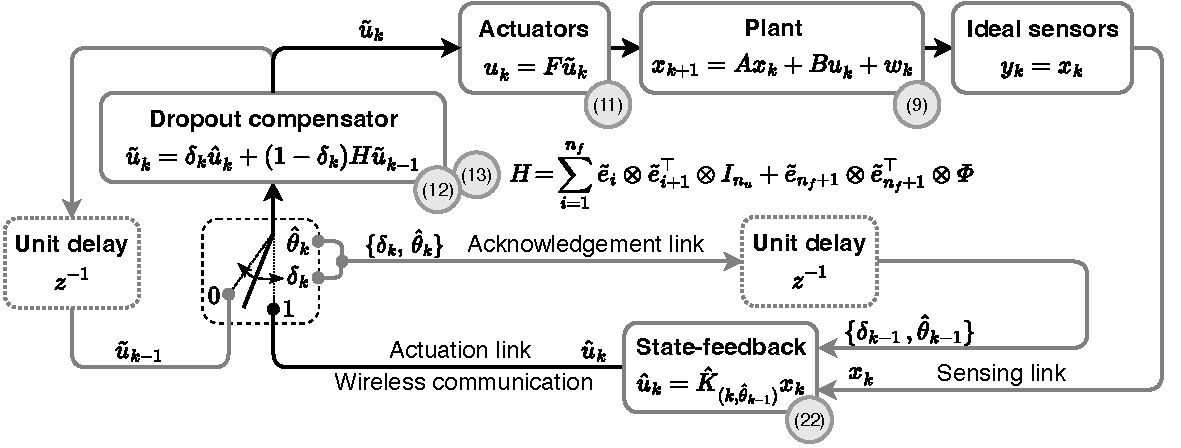
\includegraphics[width=0.8\columnwidth]{../wncs-lcss-cdc-25-architecture.pdf}
\caption{\textcolor{blue}{The closed-loop system architecture. The square blocks indicate the main components, and the shaded circles reference the related equations. A wireless link delivers SF control inputs to the actuators. The receiver measures the link state $\theta_k$ and communicates the measurement $\hat{\theta}_k$ with the transmission outcome $\delta_k$ to the controller. }}\label{fig:architecture}
\end{center}
\end{figure}
\\[4mm]
%%%
\textbf{Reviewer 9—Comment 3—}\textit{%
If LQR is used as the feedback controller, if T is infinite, we can get the control gain K offline, there is no need to discuss about the number of transferred future control inputs.}\\[2mm]
\textbf{Authors' response 3:} \textcolor{black}{
We thank the Reviewer for the observation. The measured channel-state-dependent control gains of the optimal infinite-horizon state-feedback (IHSF) controller are typically computed offline. However, these gains depend on the number of future control inputs transmitted to the actuators and the MDC scheme. Specifically, each of the $M$ IHSF gains $\hat{K}_{(\infty,\hat{s}_{\mu})}$ in (39) can be computed using (50a) in combination with (31), (32), and (49). Each IHSF control gain $\hat{K}_{(\infty,\hat{s}_{\mu})}$ in (39) comprises $n_f+1$ components $K_{(f,\hat{s}_{\mu})}$,  $f\in\mathbb{Z}^{0+}$, $f\leq n_f$, necessary for computing the control messages $\hat{u}_k$. These messages include future control inputs stored in the MDC buffer to be used in the event of subsequent control message dropouts. Each transmitted control message can be corrupted by the wireless communication link and discarded by the receiver. The MDC scheme then decides which control signal to pass as input to the actuators. The MDC decision rule (13) has $n_f$ and $\mathit{\Phi}$ as parameters. Thus, discussing future control inputs in each message obtained with the IHSF control scheme is relevant and necessary. The only way to avoid discussing the number of future control inputs and the MDC strategy is to prevent the (wireless) communication between the controller and actuators. Nevertheless, colocating the controller and actuators may be unfeasible or undesirable in several application scenarios, which motivates wireless networked control systems and this letter.}\\[4mm]
%%%
\textbf{Reviewer 9—Questions on parameter tuning—1)}\textit{ %
Why the matrix a covariance matrix $\Sigma_{w}=2.5\cdot 10^{-9} I_4$ is selected too small in simulation?}\\[2mm]
\textbf{Authors' response on parameter tuning question 1:} \textcolor{black}{We thank the Reviewer for the relevant question. All the parameters including the value of the covariance matrix $\Sigma_{w}=2.5\cdot 10^{-9} I_4$ are taken from [4] as it describes extensive Monte Carlo simulations for both finite- and infinite-horizon settings in a baseline case of no future control inputs and perfect CSI under a
link model that relies on an accurate representation of a realistic wireless communication protocol. To address the Reviewer's concern regarding the process noise possibly being too small, we consider $\Sigma_{w}=4\cdot 10^{-6} I_4$, which corresponds to a standard deviation of $0.002$ rad or rad/s, that is, $0.1146$ $^{\circ}$ or $^{\circ}\!$/s. This change affects the long-run average cost shown in Fig. 3 and discussed in the response to the next question about parameter tuning. Because the revised version of the letter adds the closed-loop system architecture in Fig. 1, the new Fig. 3 relates to Fig. 2 of the previous version.}\\[4mm]
%%%
\textbf{Reviewer 9—Questions on parameter tuning—2)}\textit{ %
If it is possible to provide a general guide of $\mathit{\Phi}$ selection? It is set $\mathit{\Phi}=0.1$ in simulation, I just wonder if different $\mathit{\Phi}$ will affect the stability and the performance of the closed-loop system. 
As the authors said in simulation: we set $\mathit{\Phi}=0.1$ as the dropout compensation factor because it provides a good trade-off between stability and control cost in the baseline case of no future control inputs and perfect CSI.} \\[2mm]
\textbf{Authors' response on parameter tuning question 2:} \textcolor{black}{We thank the Reviewer for the pertinent question. The baseline case of no future control inputs and perfect CSI was addressed in [4], where the impact of the dropout compensation factor $\mathit{\Phi}$ is examined in Section 7.6. Figures 12 and 13 from [4] depict the spectral radius of the stability verification matrix $\mathit{\Lambda}$ and the long-run average cost $J_{\infty}^{\star}$ as functions of the dropout compensation factor $\mathit{\Phi}$ for the considered linearized model of a rotary inverted pendulum in the baseline case. For the Reviewer's convenience, we show these figures below, updated for the process noise $\Sigma_{w}=4\cdot 10^{-6} I_4$. \\
% \setcounter{figure}{11}
\begin{figure}[h!]
\begin{center}
\includegraphics[width=0.7\columnwidth]{stability-cntrl-2.pdf}
%\includegraphics[width=0.7\columnwidth]{./responses-rev-1/stability-cntrl-2.pdf}
\caption{The spectral radius of the mean-square stability verification matrix, $\rho(\mathit{\Lambda})$, as a function of the dropout compensation factor $\mathit{\Phi}$ for the rotary inverted pendulum under the proposed infinite-horizon linear–quadratic regulation (LQR) [4—Fig. 12]}\label{fig:stability-coeff}
\end{center}
\end{figure}
\begin{figure}[h!]
\begin{center}
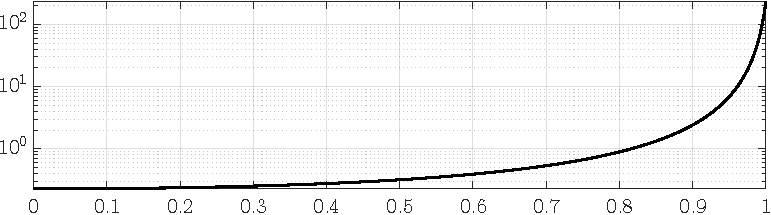
\includegraphics[width=0.7\columnwidth]{cost-cntrl-2.pdf}
\caption{Long-run average cost $J_{\infty}^{\star}(\mathit{\Phi})$ for the rotary inverted pendulum under the proposed infinite-horizon LQR for $\Sigma_{w}=4\cdot 10^{-6} I_4$. See [4—Fig. 13] for similar results, obtained with $\Sigma_{w}=2.5\cdot 10^{-9} I_4$.}\label{fig:cost-coeff}
\end{center}
\end{figure}
\begin{figure}[h!]
\begin{center}
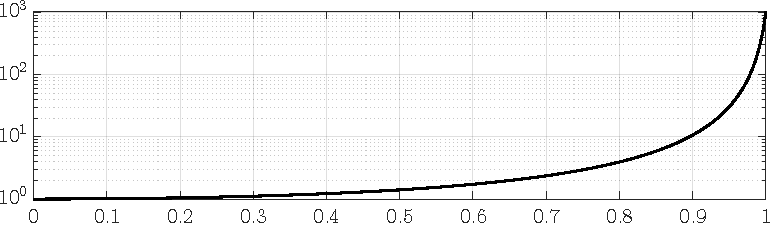
\includegraphics[width=0.7\columnwidth]{cost-ratio-2.pdf}
\caption{The ratio $\frac{J_{\infty}^{\star}(\mathit{\Phi})}{J_{\infty}^{\star}(\mathit{0})}$ for the rotary inverted pendulum with $\Sigma_{w}=4\cdot 10^{-6} I_4$.}\label{fig:cost-ratio}
\end{center}
\end{figure}\\[-4mm]
Figure \ref{fig:stability-coeff} shows that the values of $\rho(\Lambda)$ decrease from $0.9837$ in $0$ to $0.9799$ in $0.921$ and then monotonically increase to $0.9928$ in $1$. This indicates that $\mathit{\Phi} = 0.921$ provides the most stable closed-loop behavior in the mean-square sense. The value of $\rho(\Lambda)<1$ indicates the convergence rate of the closed-loop system to the mean-square stable steady state, as discussed in the response to Comment 3 of Reviewer 16. Therefore, the lower values of $\rho(\Lambda)$ are desirable, and $\mathit{\Phi} = 0.1$ produces $\rho(\Lambda)=0.9832$, which is slightly lower than $0.9837$, obtained for $\mathit{\Phi} = 0$. Furthermore, all admissible values of $\mathit{\Phi}$ produce mean-square stable system behavior, though with different long-run average costs.\\
The long-run average cost $J_{\infty}^{\star}$ for $\Sigma_{w}=4\cdot 10^{-6} I_4$ in Figure \ref{fig:cost-coeff} increases monotonically in $\mathit{\Phi}$, passing from $0.22654$ in $0$ to $0.22923$ in $0.1$, $0.23715$ in $0.2$, $0.25193$ in $0.3$, $0.27676$ in $0.4$,
$0.31823$ in $0.5$, $0.39114$ in $0.6$, $0.53508$ in $0.7$, $0.89246$ in $0.8$, 
$2.41235$ in $0.9$, and $232.55649$ in $1$. Similar results are shown in [4] in Figure 13 for $\Sigma_{w}=2.5\cdot 10^{-9} I_4$. \\
Figure \ref{fig:cost-ratio} presents the ratio of long-run average cost $J_{\infty}^{\star}$ in $\mathit{\Phi}$ to $J_{\infty}^{\star}$ in $0$, indicating an increase of three orders of magnitude in the cost for $\mathit{\Phi}=1$ compared to $\mathit{\Phi}=0$. For $\mathit{\Phi}=0.1$, the long-run average cost $J_{\infty}^{\star}$ is close to the cost in $\mathit{\Phi}=0$. \\
The long-run average cost and mean-square stability analyses in [4] reveal that the dropout compensation factors, ranging from $0$ to $0.921$, provide a trade-off between the two metrics, with particular choices depending on the design's priorities. The choice of $\mathit{\Phi} = 0.1$ presents a compelling alternative to the zero-input message dropout compensation (MDC) strategy ($\mathit{\Phi} = 0$) by offering a slightly higher cost but faster convergence to the steady state. The hold-input MDC ($\mathit{\Phi} = I$) yields mean-square stable closed-loop system behavior at a significantly higher cost. \\
The analysis above refers to the baseline case of no future control inputs and perfect CSI. The results of this letter enable analyses under imperfect CSI and a hybrid MDC that combines the transmission of multiple control inputs with the scaling of inputs to actuators when necessary. Although the space constrains of an L-CSS letter prevent us from discussing the effects of different scaling factors $\mathit{\Phi}$, we present the spectral radius of the mean-square stability verification matrix $\rho(\mathit{\Lambda})$ and the long-run average cost $J_{\infty}^{\star}$ as a function of the number of future controls $n_f$ for the three most significant values of the dropout compensation factor $\mathit{\Phi}$ ($0$, $0.921$, and $1$ from the baseline case), in addition to the case of $\mathit{\Phi}=0.1$, in the figures below.
\begin{figure}[h!]
\begin{center}
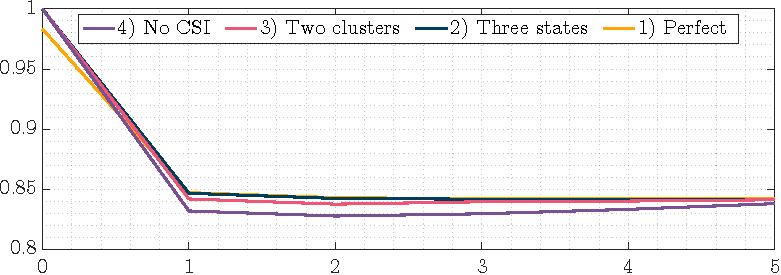
\includegraphics[width=0.76\columnwidth]{../stability-cntrl-a.pdf}
\caption{The spectral radius of the mean-square stability verification matrix, $\rho(\mathit{\Lambda})$, as a function of the number of control inputs $n_f$ for the rotary inverted pendulum under the proposed infinite-horizon linear–quadratic regulation (LQR) with the dropout compensation factor $\mathit{\Phi}=0.1$—Fig. 2 in the revised version of the letter}\label{fig:stability-coeff-a}
\end{center}
\end{figure}
\begin{figure}[h!]
\begin{center}
\includegraphics[width=0.76\columnwidth]{../cost-cntrl-a.pdf}
\caption{The long-run average cost, $J_{\infty}^{\star}$, as a function of the number of control inputs $n_f$ for the rotary inverted pendulum under the proposed infinite-horizon linear–quadratic regulation (LQR) with the dropout compensation factor $\mathit{\Phi}=0.1$—Fig. 3 in the revised version of the letter}\label{fig:cost-cntrl-a}
\end{center}
\end{figure}
\begin{figure}[h!]
\begin{center}
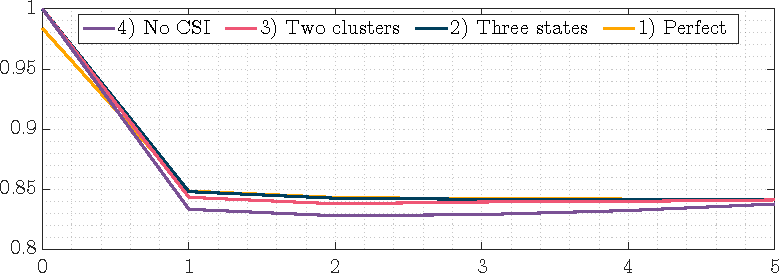
\includegraphics[width=0.76\columnwidth]{stability-cntrl-0.pdf}
\caption{The spectral radius of the mean-square stability verification matrix, $\rho(\mathit{\Lambda})$, as a function of the number of control inputs $n_f$ for the rotary inverted pendulum under the proposed infinite-horizon linear–quadratic regulation (LQR) with the dropout compensation factor $\mathit{\Phi}=0$}\label{fig:stability-coeff-0}
\end{center}
\end{figure}
\newpage
\begin{figure}[h!]
\begin{center}
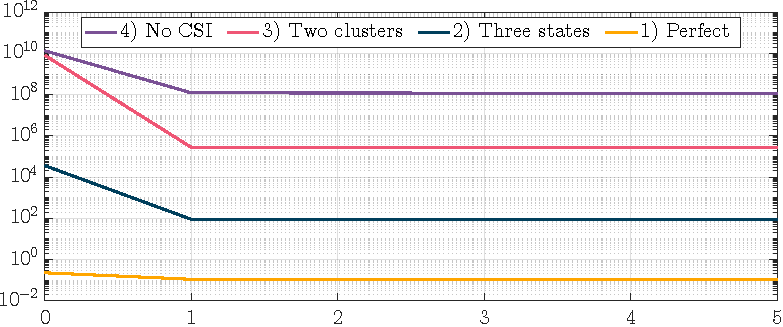
\includegraphics[width=0.76\columnwidth]{cost-cntrl-0.pdf}
\caption{The long-run average cost, $J_{\infty}^{\star}$, as a function of the number of control inputs $n_f$ for the rotary inverted pendulum under the proposed infinite-horizon linear–quadratic regulation (LQR) with the dropout compensation factor $\mathit{\Phi}=0$}\label{fig:cost-cntrl-0}
\end{center}
\end{figure}
\begin{figure}[h!]
\begin{center}
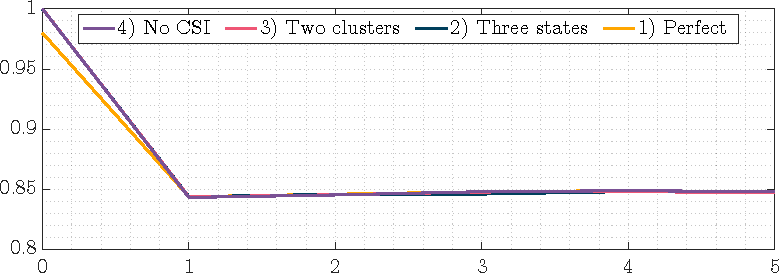
\includegraphics[width=0.76\columnwidth]{stability-cntrl-9.pdf}
\caption{The spectral radius of the mean-square stability verification matrix, $\rho(\mathit{\Lambda})$, as a function of the number of control inputs $n_f$ for the rotary inverted pendulum under the proposed infinite-horizon linear–quadratic regulation (LQR) with the dropout compensation factor $\mathit{\Phi}=0.921$}\label{fig:stability-coeff-9}
\end{center}
\end{figure}
\begin{figure}[h!]
\begin{center}
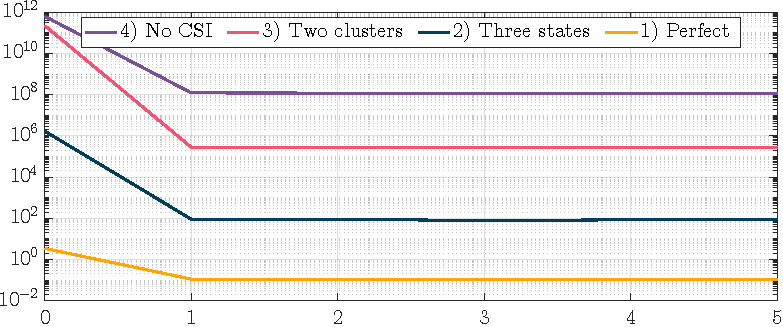
\includegraphics[width=0.76\columnwidth]{cost-cntrl-9.pdf}
\caption{The long-run average cost, $J_{\infty}^{\star}$, as a function of the number of control inputs $n_f$ for the rotary inverted pendulum under the proposed infinite-horizon linear–quadratic regulation (LQR) with the dropout compensation factor $\mathit{\Phi}=0.921$}\label{fig:cost-cntrl-9}
\end{center}
\end{figure}
\newpage
\begin{figure}[h!]
\begin{center}
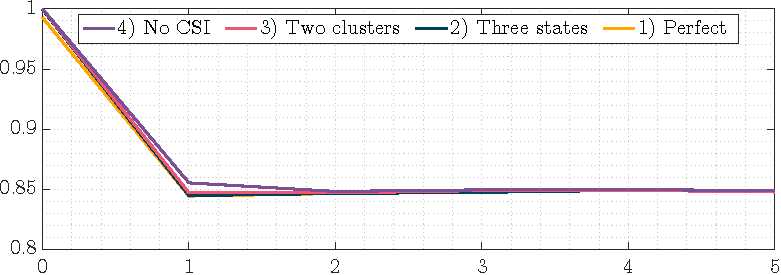
\includegraphics[width=0.76\columnwidth]{stability-cntrl-1.pdf}
\caption{The spectral radius of the mean-square stability verification matrix, $\rho(\mathit{\Lambda})$, as a function of the number of control inputs $n_f$ for the rotary inverted pendulum under the proposed infinite-horizon linear–quadratic regulation (LQR) with the dropout compensation factor $\mathit{\Phi}=1$}\label{fig:stability-coeff-1}
\end{center}
\end{figure}
\begin{figure}[h!]
\begin{center}
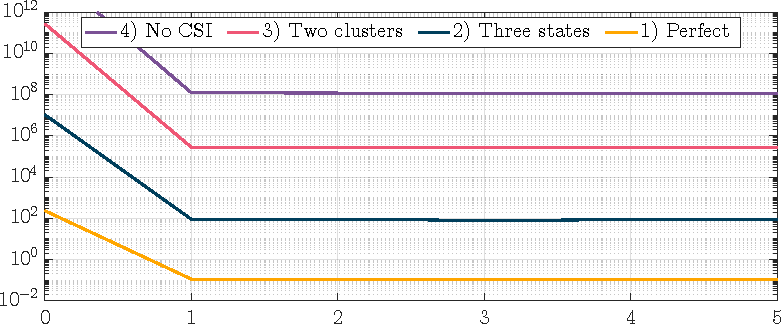
\includegraphics[width=0.76\columnwidth]{cost-cntrl-1.pdf}
\caption{The long-run average cost, $J_{\infty}^{\star}$, as a function of the number of control inputs $n_f$ for the rotary inverted pendulum under the proposed infinite-horizon linear–quadratic regulation (LQR) with the dropout compensation factor $\mathit{\Phi}=1$}\label{fig:cost-cntrl-1}
\end{center}
\end{figure}
}
\textcolor{black}{Figures \ref{fig:stability-coeff-a} and \ref{fig:cost-cntrl-a} correspond to Figures 2 and 3 in the revised version of the letter. By comparing Figure \ref{fig:stability-coeff-a} to Figure \ref{fig:stability-coeff-0} and Figure \ref{fig:cost-cntrl-a} to Figure \ref{fig:cost-cntrl-0}, we observe that differences between the closed-loop system characteristics under the MDC factors $\mathit{\Phi}$ of $0$ and $0.1$ are marginal. Our choice to present the case of $\mathit{\Phi}=0.1$ is motivated by its generality, as the zero-input MDC ($\mathit{\Phi}=0$) is a very special case that requires less complex analysis. The closed-loop system with $\mathit{\Phi}=0.1$ has slightly better performance in terms of stability at the price of a slightly worse long-run average cost.\\
Similar to the baseline case, Figures \ref{fig:stability-coeff-a}–\ref{fig:cost-cntrl-1} show that the MDC factor $\mathit{\Phi}=0.921$ yields the most stable closed-loop system for all considered numbers of control inputs, $n_f$, at significantly higher long-run average costs (Figures \ref{fig:stability-coeff-9} and \ref{fig:cost-cntrl-9}). The hold-input MDC strategy ($\mathit{\Phi}=1$) ensures stable closed-loop system behavior; however, it has the lowest convergence rate and the highest long-run average cost, making it less desirable in terms of performance (Figures \ref{fig:stability-coeff-1} and \ref{fig:cost-cntrl-1}).} \\[4mm]
%%%
\textbf{Reviewer 9—Questions on notations—1)}\textit{ %
What is the difference between $u^{n_f}_T$ in Eq. (15) and $\bar{u}$ in Eq (10). What is the definition on $f$ in Eq (15). It is a little bit mess in notations. I suggest you to check it through all letter.}\\[2mm]
\textbf{Authors' response on parameter tuning question 1:} \textcolor{black}{We thank the Reviewer for the question. Equation (15) is a part of a sentence stating that ``$\bm{u}_{T}^{n_f}$ is a sequence of length $T$ of control messages as in (10) such that $\bar{u}_{(k+f\mid k)} = K_{(k+f,\hat{\theta}_{k-1})}x_k$.'' This statement means that (15) provides a constraint for a generic control message $\hat{u}_k$ defined by (10), where $\hat{u}_k = \big([\bar{u}_{(k+f\mid k)}^{\top}]_{f=0}^{n_f}\big)^{\!\top}$. 
The meaning of $f$ becomes self-explanatory from substituting the generic elements $\bar{u}_{(k+f\mid k)}$ of the control message $\hat{u}_k$ in (10) with their specific definition in (15):
$\hat{u}_k = \Big([(K_{(k+f,\hat{\theta}_{k-1})}x_k)^{\top}]_{f=0}^{n_f}\Big)^{\!\top}$. In words, $f$ indexes the elements of the control message, % at time $k$, 
with $f=0$ indicating the current input, and $f\geq 1$ pinpointing specific future inputs. The meaning of $f$ never changes throughout this letter, and the notation is consistent. 
$f \in \mathbb{Z}^{0+}$ and $f\leq n_f$ in (10), (22), and (39). Finally, this letter uses parenthesis to identify sequences. Thus, $\bm{u}_{T}^{n_f}$ can be expressed as $\bm{u}_{T}^{n_f} = (\hat{u}_k)_{k=0}^{T-1}$, where $\hat{u}_k$ is defined by (10) and each element of $\hat{u}_k$ satisfies (15). 
}\\[4mm]
%%%
\textbf{Reviewer 9—Questions on notations—2)}\textit{ %
Where is the definition of $\mathbb{B}$ in Eq. (29)?}\\[2mm]
\textbf{Authors' response on parameter tuning question 2:} \textcolor{black}{We thank the Reviewer for the question. If the Reviewer refers to $\mathcal{B}$, it is defined by equation (31), which is shown at the top of page 5, as indicated by the sentence that follows equation (29). There is no $\mathbb{B}$ in this letter.}\\[4mm]
%%%
\textbf{Reviewer 9—Other suggestion on expression—1)}\textit{ %
Abbreviation of linear–quadratic regulators (LQR) should be added for highlight in introduction.}\\[2mm]
\textbf{Authors' response to the first suggestion on expression:} \textcolor{black}{
We thank the Reviewer for the suggestion. In the introduction, we refrain from using the abbreviation LQR for linear–quadratic regulators to avoid confusing it with different, albeit related, meanings, as we utilize LQR to refer specifically to linear–quadratic regulation in Section 3 and beyond.}\\[4mm]
%%%
\textbf{Reviewer 9—Other suggestion on expression—2)}\textit{ %
The sequences in Eq. (14) are suggested to expressed as $[x_t]^k_{t=0}$, instead of $(x_t)^k_{t=0}$ for example.}\\[2mm]
\textbf{Authors' response to the second suggestion on expression:} \textcolor{black}{We thank the Reviewer for the suggestion. This letter follows the notation of [4], % \cite{yZL-2025-automatica}, 
where curly brackets enclose the values of sets, square brackets define matrices, and parentheses identify sequences. Thus, we refrain from using square brackets to define sequences to avoid confusion between sequences and matrices.}\\[4mm]
%%%
\textbf{Authors' concluding remark:} \textcolor{black}{We are grateful to the Reviewer for the comments and suggestions. We sincerely hope the above explanations have adequately addressed the Reviewer's concerns.}
% \putbib
% \end{bibunit}
\section{Response to Reviewer 10}
% \begin{bibunit}
\textbf{Reviewer 10---Major Contribution of the Paper---}\textit{%
This letter proposes a novel framework to address the issue of imperfect CSI in WNCS and presents solutions under both finite- and infinite-horizon LQR formulations.}\\[2mm]
\textbf{Authors' response:} \textcolor{black}{We truly appreciate the Reviewer's careful reading of our paper and valuable comments. In the revised version, we have carefully addressed the Reviewer's concerns and made the required modifications.}\\[4mm]
%%%
\textbf{Reviewer 10---Organization and Style---}\textit{%
The letter is well-organized and logically structured, but some descriptions could be more readable.
For example, in Part II, the paragraph beginning with ``Wireless receivers perform CSI measurements...'' could be improved by describing the signal flow explicitly: e.g., what information is transmitted from the sensor to the controller at time step $k$, then from the controller to the actuator, and how the detector provides the controller with the measured CSI from step $k-1$, etc.}\\[2mm]
\textbf{Authors' response:} \textcolor{black}{We thank the Reviewer for this valuable comment, which helped us improve the clarity of our letter. Due to space constraints, we could only provide a concise overview of the closed-loop system architecture in Fig. 1, which has been added to Section III in the revised version of the letter, immediately after describing the system model. The related excerpt of the revised version of the manuscript is included below for the Reviewer's convenience.}\\
\textcolor{blue}{Fig.~\ref{fig:architecture} summarizes this closed-loop system architecture.}
\begin{figure}[h!]
\begin{center}
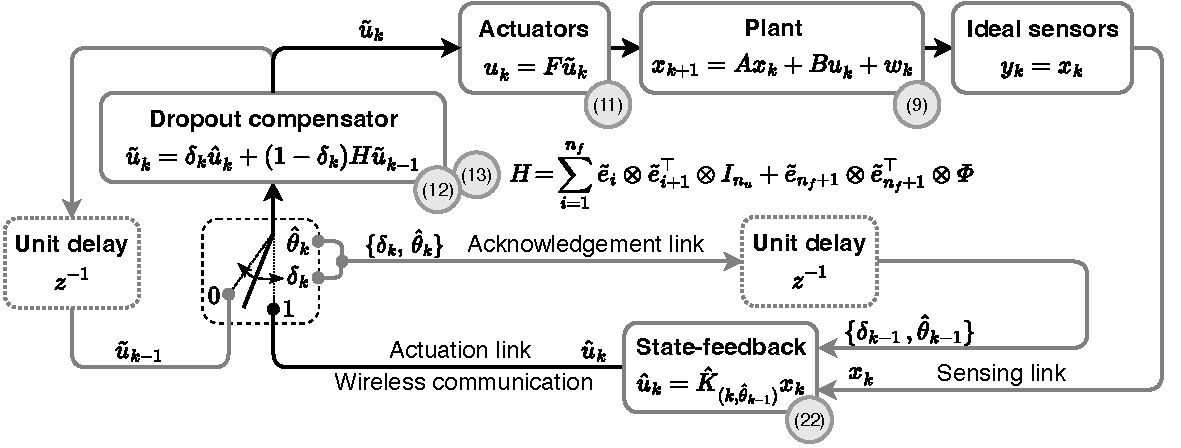
\includegraphics[width=0.8\columnwidth]{../wncs-lcss-cdc-25-architecture.pdf}
\caption{\textcolor{blue}{The closed-loop system architecture. The square blocks indicate the main components, and the shaded circles reference the related equations. A wireless link delivers SF control inputs to the actuators. The receiver measures the link state $\theta_k$ and communicates the measurement $\hat{\theta}_k$ with the transmission outcome $\delta_k$ to the controller. }}\label{fig:architecture}
\end{center}
\end{figure}\\[2mm]
%%%
\textbf{Reviewer 10---Technical Accuracy---1)}\textit{ %
Several variables are not explicitly defined in the text, such as $H^i$ in equation (23).}\\[2mm]
\textbf{Authors' response:} \textcolor{black}{We appreciate the Reviewer's feedback. We checked the manuscript for the definitions of the variables. $H$ refers to the message dropout compensation (MDC) scheme formalized by equation (13) and described in the text below the equation. Similar to $A^{h-i}$, $H^{i}$ in (23) indicates matrix exponentiation. It produces the following matrices.}
\begin{equation*}
    n_f = 0 \Rightarrow H^0 = I_{n_u},~H^1 = H = \mathit{\Phi},~H^2 = \mathit{\Phi}^{2},\dots,~H^i= \mathit{\Phi}^i~\forall i\in\mathbb{Z}^{0+}.
\end{equation*}
\begin{equation*}
    n_f = 1 \Rightarrow H^0 = \begin{bmatrix} I_{n_u} & 0 \\ 0 & I_{n_u} \end{bmatrix},~H^1 = H = \begin{bmatrix} 0 & I_{n_u} \\ 0 & \mathit{\Phi} \end{bmatrix},~H^2 = \begin{bmatrix} 0 & \mathit{\Phi} \\ 0 & \mathit{\Phi}^2 \end{bmatrix},\dots,
    ~H^i = \begin{bmatrix} 0 & \mathit{\Phi}^{i-1} \\ 0 & \mathit{\Phi}^i \end{bmatrix}~\forall i\in\mathbb{Z}^{+}.
\end{equation*}
\begin{equation*}
    n_f = 2 \Rightarrow H^0 =\! \begin{bmatrix} I_{n_u} & 0 & 0 \\ 0 & I_{n_u} & 0 \\ 0 & 0 & I_{n_u} \end{bmatrix}\!,~H^1 = H =\! \begin{bmatrix} 0 & I_{n_u} & 0 \\ 0 & 0 & I_{n_u} \\ 0 & 0 & \mathit{\Phi} \end{bmatrix}\!,\dots,
    ~H^i =\! \begin{bmatrix} 0 & 0 & \mathit{\Phi}^{i-2} \\ 0 & 0 & \mathit{\Phi}^{i-1} \\ 0 & 0 & \mathit{\Phi}^i \end{bmatrix}\!,
    ~\forall i\in\mathbb{Z}^{+}, i\geq 2. 
\end{equation*}
The explicit versions of $H^i$ matrices for $n_f>2$ follow the pattern defined by (13) and matrix multiplication. Due to the strict page limit of an L-CSS letter, we could not include any of these explicit forms in the revised version of the manuscript.\\[4mm]
%%%
\textbf{Reviewer 10---Technical Accuracy---2)}\textit{ %
In equation (5b), the summation over $\alpha_{i\mu}$ should
be with respect to $\mu$, not $i$, to ensure that the sum of the probabilities of all possible detector outputs given the true channel state $s_i$ is 1 --- consistent with the notation in equation (1).}\\[2mm]
\textbf{Authors' response:} \textcolor{black}{We are grateful to the Reviewer for this helpful observation. The Reviewer is correct: the summation over $\alpha_{i\mu}$ should be in $\mu$. We have corrected this typo in the revised version of the manuscript. This typo did not affect the other equations or the numerical implementation used to obtain the results in Section VIII. The revised equation (5b) version follows for the Reviewer's convenience.}
\begin{equation*}
   \mathbb{P}(\hat{\theta}_{k} = \hat{s}_{\mu} \mid \theta_{k} = s_i) = \alpha_{i\mu} \geq 0,~ \textcolor{blue}{\sum_{\mu=1}^M \alpha_{i\mu}= 1}.
\end{equation*}
\\[2mm]
%%%
\textbf{Reviewer 10---Technical Accuracy---3)}\textit{ %
Additionally, Part VIII does not specify whether the numerical example corresponds to the finite- or infinite-horizon case.}\\[2mm]
\textbf{Authors' response:} \textcolor{black}{We thank the Reviewer for the observation. This information is implicitly provided in the first sentence of the last paragraph of Section VIII: ``To compare the effects of transmitting several future control inputs on stability and control cost, we solve the LMIs (49) in the same setting.'' The state-feedback control gains are obtained by solving the LMIs (49), which refer to the infinite-horizon case addressed in Section VII. The stability issues also refer to the infinite-horizon setting, as discussed in Section VI. Unfortunately, we cannot explicitly indicate the infinite-horizon case without exceeding the rigid six-page limit of an L-CSS letter. On a side note, the finite-horizon state-feedback control for the baseline case of no future control inputs and perfect CSI is extensively validated by a statistically significant number of Monte Carlo simulations in [4].}\\[4mm]
%%%
\textbf{Reviewer 10---Technical Accuracy---4)}\textit{ %
In Figures 1 and 2, it's unclear why 3) is labeled as clusters while 4) is states. Since ``perfect" effectively corresponds to 4 clusters, perhaps the ordering should follow the degree of CSI quality: perfect, three, two, no CSI.}\\[2mm]
\textbf{Authors' response:} \textcolor{black}{We sincerely appreciate the Reviewer's pertinent comment. Because of the deadline for the initial submission and the rigid space constraints of an L-CSS letter, we have omitted details of the four scenarios analyzed in the numerical example. We integrated these details in the revised version of the letter, as reported below, for the Reviewer's convenience.}\\
``Fig. 3 shows the corresponding control costs in four selected scenarios: \textcolor{blue}{1) Perfect CSI; 2) Three measured states with thresholds $\{\hat{\beta_i}\}_{i=1}^{2} \!=\! \{-2.98,-2.08\}\,$dB and Gaussian CSI measurement noise having $\sigma_{\omega}^2=10^{-4}$; 3) Two clusters with a threshold $\hat{\beta}_1\!=\!-2.55\,$dB without CSI measurement noise; 4) No CSI.}''\\
\textcolor{black}{This information helps us to address the Reviewer's comment properly. The clusters refer to non-overlapping groups of states, i.e., disjoint sets of states. Thus, scenarios 1), 3), and 4) involve clusters. Specifically, the perfect CSI scenario 1) has $M=N=4$ and $P_e = I_N$, with four states belonging to separate clusters. Scenario 3) has the SINR threshold of $-2.55\,$dB, which coincides with the FSMC threshold $\beta_2$. Consequently, the first cluster comprises the FSMC states $s_1$ and $s_2$, while the second includes $s_3$ and $s_4$. The corresponding emission probability matrix (EPM) is 
\begin{equation*}
P_e=\begin{bmatrix}
1 & 0 \\ 1 & 0 \\ 0 & 1 \\ 0 & 1
\end{bmatrix}.
\end{equation*}
Scenario 4) has only one cluster with all FSMC states and $P_e=\bm{1}$. However, Scenario 2) has a detector with three output states, each including overlapping FSMC states owing to different SINR thresholds. Its EPM is 
\begin{equation*}
P_e=\begin{bmatrix}
1 & 0 & 0 \\ 0.337 & 0.663 & 0 \\ 0 & 0.613 & 0.387 \\ 0 & 0 & 1
\end{bmatrix}.
\end{equation*}
In conclusion, we have followed the Reviewer's suggestion and listed the scenarios in decreasing order of the detector's state number, from 4 to 1. As detailed above, the cluster keyword indicates a non-overlapping grouping of the FSMC states into sets and cannot be applied to the second scenario. For the Reviewer's convenience, we have reported the updated figures below. Please note a change in the long-run average costs because of the different process noise covariance requested by Reviewer 9.}
\begin{figure}[h!]
\begin{center}
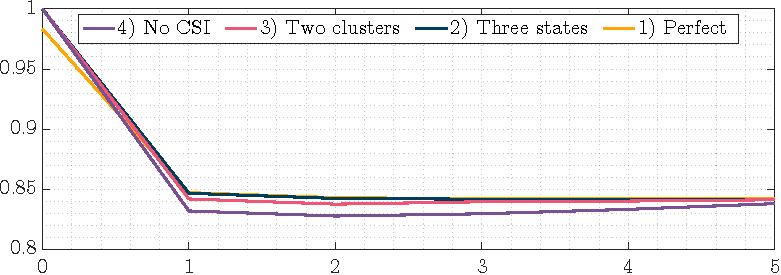
\includegraphics[width=0.76\columnwidth]{../stability-cntrl-a.pdf}
\caption{$\rho(\mathit{\Lambda})$ from (48) as a function of $n_f$.}\label{fig:stability}
\end{center}
\end{figure}
\begin{figure}[h!]
\begin{center}
\includegraphics[width=0.76\columnwidth]{../cost-cntrl-a.pdf}
\caption{The long-run average cost $J_{\infty}^{\star}$ from (50b) as a function of $n_f$.}\label{fig:cost}
\end{center}
\end{figure}
\\[4mm]
%%%
\textbf{Reviewer 10---Technical Accuracy---5)}\textit{ %
The claim that ``one future control input provides the most significant improvement'' --- is this generally true?}\\[2mm]
\textbf{Authors' response:} \textcolor{black}{We thank the Reviewer for the question. All the considerations regarding $\rho(\mathit{\Lambda})$ and $J_{\infty}^{\star}$ values in Section VIII refer to the presented linearized model of a rotary inverted pendulum controlled over a specific FSMC and have no general validity, i.e., transmitting more than one future control input may be helpful in different settings. The theoretical results of this letter enable answering the question of the most suitable number of future control inputs to transmit for any linear plant, FSMC, EPM, and message dropout compensation matrix $\mathit{\Phi}$. Please see our response to Reviewer 9's second question on parameter tuning for an example that considers different values $\mathit{\Phi}$.
}\\[4mm]
%%%
\textbf{Reviewer 10---Technical Accuracy---6)}\textit{ %
If the four channel states had higher packet loss rates, could it be possible that sending more future control inputs would become more beneficial?}\\[2mm]
\textbf{Authors' response:} \textcolor{black}{We thank the Reviewer for the question. In principle, sending additional future control inputs may be more beneficial in scenarios with an exceptionally high message dropout rate. However, we did not find any examples supporting this. Our letter presented a setting with a high average message dropout probability (AMDP) of $9.075$\% and neglected the increase in dropout probability due to increased message length. As an example of the effects of the number of future control inputs that account for the message length increase and much higher average message dropout probabilities, consider the same plant model in a setting with $18$ Wi-Fi devices operating under saturated conditions, all located $7.5$ meters from the control message receiver, which is positioned $5$ meters away from the controller. The closed-loop control relies on the ISA-100.11a. Other parameters can be found in [12]. The resulting four-state Markov channels are as follows. The subscript index indicates the number of future control inputs that yield the reported TPM and the corresponding vectors of successful message delivery probabilities.
\begin{equation*}
    P_{c.0} = 
\begin{bmatrix}
0.232 & 0.025 & 0.030 & 0.713 \\
0.212 & 0.024 & 0.028 & 0.736 \\
0.210 & 0.024 & 0.028 & 0.738 \\
0.175 & 0.022 & 0.026 & 0.777
\end{bmatrix},~
\hat{\delta}_{.0} = 
\begin{bmatrix}
0.022 \\ 0.374 \\ 0.633 \\ 0.991
\end{bmatrix}^{\top},~\text{AMDP}_{0} = 21.418\%.
\end{equation*}
\begin{equation*}
    P_{c.1} = 
\begin{bmatrix}
0.236 & 0.025 & 0.029 & 0.710 \\
0.216 & 0.024 & 0.028 & 0.732 \\
0.213 & 0.024 & 0.028 & 0.735 \\
0.179 & 0.021 & 0.025 & 0.775
\end{bmatrix},~
\hat{\delta}_{.1} = 
\begin{bmatrix}
0.021 \\ 0.374 \\ 0.633 \\ 0.991
\end{bmatrix}^{\top},~\text{AMDP}_{1} = 21.798\%.
\end{equation*}
\begin{equation*}
    P_{c.2} = 
\begin{bmatrix}
0.240 & 0.025 & 0.029 & 0.706 \\
0.220 & 0.024 & 0.028 & 0.728 \\
0.217 & 0.023 & 0.028 & 0.732 \\
0.182 & 0.021 & 0.025 & 0.772
\end{bmatrix},~
\hat{\delta}_{.2} = 
\begin{bmatrix}
0.020 \\ 0.374 \\ 0.633 \\ 0.991
\end{bmatrix}^{\top},~\text{AMDP}_{2} = 22.132\%.
\end{equation*}
\begin{equation*}
    P_{c.3} = 
\begin{bmatrix}
0.243 & 0.024 & 0.029 & 0.704 \\
0.223 & 0.023 & 0.028 & 0.726 \\
0.220 & 0.023 & 0.027 & 0.730 \\
0.185 & 0.021 & 0.025 & 0.769
\end{bmatrix},~
\hat{\delta}_{.3} = 
\begin{bmatrix}
0.020 \\ 0.374 \\ 0.633 \\ 0.991
\end{bmatrix}^{\top},~\text{AMDP}_{3} = 22.430\%.
\end{equation*}
\begin{equation*}
    P_{c.4} = 
\begin{bmatrix}
0.246 & 0.024 & 0.028 & 0.702 \\
0.226 & 0.023 & 0.027 & 0.724 \\
0.223 & 0.023 & 0.027 & 0.727 \\
0.188 & 0.021 & 0.025 & 0.766
\end{bmatrix},~
\hat{\delta}_{.4} = 
\begin{bmatrix}
0.019 \\ 0.374 \\ 0.633 \\ 0.991
\end{bmatrix}^{\top},~\text{AMDP}_{4} = 22.699\%.
\end{equation*}
\begin{equation*}
    P_{c.5} = 
\begin{bmatrix}
0.249 & 0.024 & 0.028 & 0.699 \\
0.228 & 0.023 & 0.027 & 0.722 \\
0.225 & 0.023 & 0.027 & 0.725 \\
0.190 & 0.021 & 0.025 & 0.764
\end{bmatrix},~
\hat{\delta}_{.5} = 
\begin{bmatrix}
0.019 \\ 0.374 \\ 0.633 \\ 0.991
\end{bmatrix}^{\top},~\text{AMDP}_{5} = 22.945\%.
\end{equation*}
Consider the four scenarios of the letter previously discussed in response to the fourth Reviewer's comment on technical accuracy. 
Figures \ref{fig:stability-coeff-x} and \ref{fig:cost-cntrl-x} illustrate the stability and long-run average cost in the presented setting, with a process noise covariance $\Sigma_w \!=\! 4\cdot 10^{-6} I_4$. Similar to the setting of the letter, transmitting one future control input offers the most significant benefit regarding stability and control cost. Transmitting two control inputs reduces $\rho(\mathit{\Lambda})$ but increases $J_{\infty}^{\star}$ compared to transmitting one future control input. 
The results concerning the fourth scenario of no CSI are limited to three future control inputs, as sending four or more future control inputs leads to instability in the closed-loop system due to extremely high message dropout rates indicated by AMDP values exceeding $22.5$\%. The values of $\rho(\mathit{\Lambda})$ become $38.543$ and $50.569$, which indicate highly unstable behavior with infinite cost. Theorem 5 is applicable only to stabilizable systems, meaning that the values of $J_{\infty}^{\star}$ cannot be obtained using (50b) for the fourth scenario of no CSI with more than three future control inputs. Due to the page limit of an L-CSS letter, we could not include these details in the revised version of the manuscript.
\begin{figure}[h!]
\begin{center}
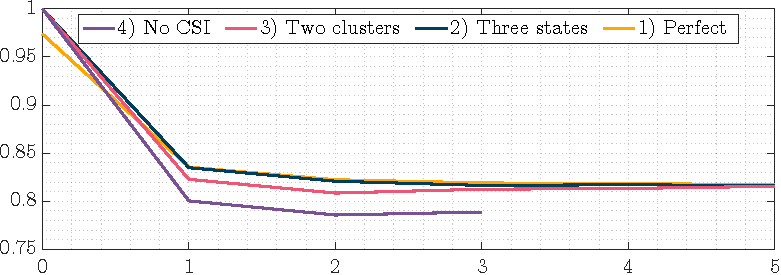
\includegraphics[width=0.76\columnwidth]{stability-cntrl-x.pdf}
\caption{The spectral radius of the mean-square stability verification matrix, $\rho(\mathit{\Lambda})$, as a function of the number of control inputs $n_f$ for the rotary inverted pendulum under the proposed infinite-horizon linear–quadratic regulation (LQR) with the dropout compensation factor $\mathit{\Phi}=0.1$ and FSMCs 1–5 described above.}\label{fig:stability-coeff-x}
\end{center}
\end{figure}
\begin{figure}[h!]
\begin{center}
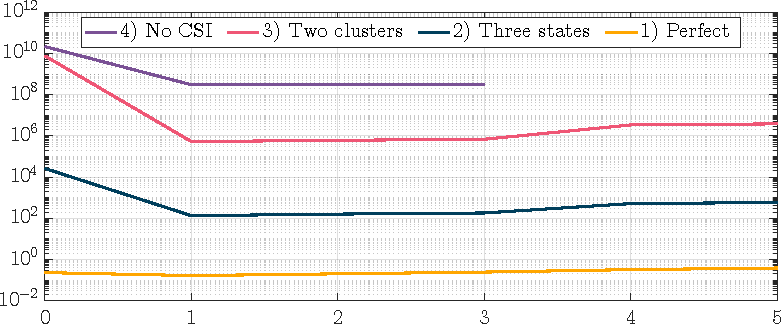
\includegraphics[width=0.76\columnwidth]{cost-cntrl-x.pdf}
\caption{The long-run average cost, $J_{\infty}^{\star}$, as a function of the number of control inputs $n_f$ for the rotary inverted pendulum under the proposed infinite-horizon linear–quadratic regulation (LQR) with the dropout compensation factor $\mathit{\Phi}=0.1$ and FSMCs 1–5 described above.}\label{fig:cost-cntrl-x}
\end{center}
\end{figure}
}\\[4mm]
%%%
\textbf{Reviewer 10---Technical Accuracy---7)}\textit{ %
Regarding the statement ``The control law without CSI performs worse regarding control costs but benefits the most from a future control input''---doesn't Figure 2 show that the ``two-cluster'' case benefits more than the ``no CSI'' case?}\\[2mm]
\textbf{Authors' response:} \textcolor{black}{We are thankful to the Reviewer for a thoughtful observation. The considered statement referred to Fig. 1 in the previous version of the manuscript, which is now Fig. 2 in the revised version of the letter, since the no CSI case has the greatest improvement in terms of $\rho(\mathit{\Lambda})$. Please note that we removed this statement to make room for the details on all four selected scenarios and the new Fig. 1, which clarifies the closed-loop system architecture. The final observations on the numerical results in Figs. 2 and 3 are reported below for the Reviewer’s convenience.}\\
\textcolor{blue}{All scenarios show that transmitting one future control input significantly improves stability and control costs, while more accurate and detailed CSI always reduces control costs.}\\[4mm]
%%%
\textbf{Reviewer 10---Presentation---}\textit{%
In Part III, the sentence ``Similarly to [4], [5]...'' should be revised. ``similarly'' $\to$ ``similar''.}\\[2mm]
\textbf{Authors' response:} \textcolor{black}{We thank the Reviewer for the valuable suggestion. We have implemented it.}\\[4mm]
%%%
\textbf{Reviewer 10---Adequacy of Citations---}\textit{%
The citations appear to be adequate.}\\[2mm]
\textbf{Authors' response:} \textcolor{black}{We are grateful to the Reviewer for the valuable feedback.}\\[4mm]
%%%
\textbf{Authors' concluding remark:} \textcolor{black}{We are thankful to the Reviewer for the valuable comments and suggestions. We sincerely hope the above explanations have adequately addressed the Reviewer's concerns.}
% \putbib
% \end{bibunit}
\section{Response to Reviewer 16}
\begin{bibunit}[alpha]
\textbf{Reviewer 16---General comments---}\textit{%
This paper addresses linear control over wireless links with imperfect channel-state information, formulating a hidden Markov jump linear system that transmits multiple future inputs with dropout compensation.
Its contributions include both finite and infinite-horizon LQR solutions and a spectral-radius-based stability condition. The manuscript is concise and well-structured. There are some comments and questions that the authors are invited to consider.}\\[2mm]
\textbf{Authors' response:} \textcolor{black}{We sincerely appreciate the Reviewer's careful reading of our paper and their valuable comments. We have addressed each of them below.}\\[4mm]
%%%
\textbf{Reviewer 16---Comment 1---}\textit{%
You introduce a parameter $L$ (the maximal number of consecutive control message dropouts) and show that for large enough dropout intervals, certain transition probabilities become negligible. 
In practice, is $L$ purely a theoretical bound, or is it also enforced by additional network constraints (e.g., maximum re-transmissions)?}\\[2mm]
\textbf{Authors' response to comment 1:} \textcolor{black}{We thank the Reviewer for the valuable comment. 
The maximal number of consecutive control message dropouts, $L$, is an intrinsic characteristic of the finite-state Markov channel (FSMC), the detector observing it, and the model reliability threshold, $\epsilon$. We use the machine epsilon as the threshold $\epsilon$ to obtain the most reliable numerical results. The emission probability matrix, $P_e$, indicates the quality of the practical channel state information (CSI), ranging from perfect CSI, which is often challenging to obtain, to no CSI. This letter follows the analytical framework from [12] to rely on the FSMC characterization at the message or packet level, meaning that the successful delivery probability (SDP) accounts for all relevant communication constraints, comprising signal-processing and diversity techniques. This includes, for instance, path diversity, channel encoding, multiple antennas, and re-transmissions. Consequently, $L$ accounts for all practical communication constraints of an FSMC that operates with the control application timing. Please refer to [12] for additional details on the FSMCs for wireless networked control systems coupled design.}\\[4mm]
%%%
\textbf{Reviewer 16---Comment 2---}\textit{%
The ergodicity assumption (A.4) ensures the existence of a steady-state probability $\pi(\infty)$ for the channel. 
Are there scenarios where $\{\theta_k\}$ is non-ergodic (e.g., absorbing states or block-fading channels)? 
How would your results be modified or extended to handle a partially ergodic or slowly time-varying model?}\\[2mm]
\textbf{Authors' response to comment 2:} \textcolor{black}{We are thankful to the Reviewer for a thoughtful comment. The ergodicity assumption (A.4) is used only in the infinite-horizon setting, addressed in Sections VI–VIII. The finite-horizon results are directly applicable to the time-varying setting if the underlying time-varying FSMC model is known. If the FSMC model is polytopic time-inhomogeneous (PTI)—that is, its transition probability matrices (TPMs) and SDP vectors are time-varying within a known polytopic set, and their exact values are unknown—the results of this letter could be extended by following the ideas of \cite{zacchialun2025lcss}. Regarding the infinite-horizon setting without the ergodicity assumption, we must distinguish between the non-ergodic and slowly time-varying cases. To our knowledge, all realistic FSMCs that operate with the control application timing are ergodic. These models incorporate block fading and do not admit absorbing states. So, we do not delve into non-ergodic settings, but we would be interested in learning about time-homogeneous non-ergodic FSMCs of practical relevance. Regarding the slowly time-varying case, our infinite-horizon analysis can be helpful if the channel variations are slower than the closed-loop system transient. If less than one, the spectral radius of the mean-square stability verification matrix, $\rho(\mathit{\Lambda})$, indicates exponential convergence rate, as detailed in our response to the Reviewer’s next question.}\\[4mm]
%%%
\textbf{Reviewer 16---Comment 3---}\textit{%
In Theorem 4, $\rho(\Lambda) < 1$ is the condition for mean-square stability. 
Beyond guaranteeing $\rho(\Lambda) < 1$, do you have insights on how quickly the states converge in practice? 
Is there a known rate of convergence or mixing time for the underlying Markov chain that
influences closed-loop transient behaviour?}\\[2mm]
\textbf{Authors' response to comment 3:} \textcolor{black}{We are grateful to the Reviewer for an excellent question. The condition $\rho(\Lambda)<1$ is necessary and sufficient for the mean-square stability (MSS) of a (hidden) Markov jump linear system (MJLS). According to the MJLS theory presented in \cite{costa2006discrete} and \cite{zacchialun2019automatica}, MSS is equivalent to exponential MSS even in the PTI setting, and the value of the (joint) spectral radius of the mean-square stability verification matrix relates to the maximal exponential decay rate. Please refer to the proofs of \cite[Prop. 3.25]{costa2006discrete} and \cite[Thm. 14, 16]{zacchialun2019automatica} for additional technical details.}\\[4mm]
%%%
\textbf{Reviewer 16---Comment 4---}\textit{%
In many industrial or mobile scenarios, channel statistics can drift over time (e.g., changes in multipath profiles, device mobility). 
Does your framework allow for slowly time-varying TPMs $P_c$ or detection matrices $P_e$?}\\[2mm]
\textbf{Authors' response to comment 4:} \textcolor{black}{We thank the Reviewer for the relevant question. As detailed in our responses to the Reviewer's previous questions, our framework allows for time-varying TPMs and SDP vectors. If TPM and SDP values are known, our finite-horizon results can be applied directly. Similar to \cite{zacchialun2025lcss}, if TPMs and SDP vectors are unknown but bounded by the known polytopic sets, the finite-horizon results could be extended to account for such a setting. The infinite-horizon theoretical results could be extended to the PTI setting via \cite{zacchialun2019automatica} and \cite{zacchialun2019ecc}, but computing the joint spectral radius over a set of relevant mean-square stability verification matrices may be currently computationally unfeasible—please see our response to the Reviewer's fifth comment for additional details. 
Finally, the infinite-horizon results presented in this letter can be applied to settings with slowly varying TPMs and SDP vectors, as long as their values are known and channel variations happen more slowly than the transients of the closed-loop system. To this end, this letter demonstrates that a careful choice of the number of future control inputs included in the controller's messages, along with the message dropout compensation strategy, can significantly reduce the value of $\rho(\Lambda)$ and shorten the transient phase of the closed-loop system. Regarding the emission probability matrices $P_e$, we would leave them constant since they represent the practical constraints of a detector and account for the general quality of available CSI. In other words, $P_e$ is a parameter of the CSI detection schemes and can be used as a wireless networked control system design parameter.}\\[4mm]
%%%
\textbf{Reviewer 16---Comment 5---}\textit{%
Could you comment on how the computational burden scales with $N$, $M$, and $n_f$? 
For instance, how feasible is the approach for larger state spaces or multiple clusters?}\\[2mm]
\textbf{Authors' response to comment 5:} \textcolor{black}{We thank the Reviewer for an excellent question. The number of discrete states of the hidden MJLS mainly determines the computational burden. This discrete state space is given by the product of $L+1$ and $M$ or $M^2$, as indicated by (25) and (42). $L$ increases with the message error rate of the FSMC and with lower model reliability thresholds $\epsilon$. For instance, this letter's numerical example considers an FSMC with a high average message dropout probability (AMDP) of 9.075\% and $\epsilon = 2.220446049250313\cdot 10^{-16}$. This setting results in $L = 27$. Setting  $\epsilon = 10^{-12}$ would lead to $L = 20$, thus reducing complexity and model reliability. $M\leq N$. Designing a controller with fewer detector states reduces the computational burden at the expense of increased control cost, as shown in Fig. \ref{fig:stability-coeff-16}, reproduced below, for the Reviewer's convenience.
\setcounter{figure}{2}
\begin{figure}[h!]
\begin{center}
\includegraphics[width=0.76\columnwidth]{cost-cntrl-a.pdf}
%\includegraphics[width=0.7\columnwidth]{./responses-rev-1/stability-cntrl-2.pdf}
\caption{The long-run average cost $J_{\infty}^{\star}$ from (50b) as a function of $n_f$.}\label{fig:stability-coeff-16}
\end{center}
\end{figure}\\
The no-CSI setting incurs the lowest computational burden, while the perfect CSI setting is the most computationally demanding. Finding an optimal infinite-horizon controller in the mode-independent (no-CSI, $M=1$) setting has a low computational burden for any given FSMC, regardless of the number of its states $N$, if $L$ is the same. This makes the mode-independent control strategy particularly appealing for scenarios with many discrete and continuous states (i.e., $N$ and $n_x$ big). Finally, $n_f+1$ is a multiplicative factor that determines the number of control inputs. It only affects the number of basic matrix operations required by (11), (13), (22), (23), and their combination in (24), which has a limited impact on overall complexity. Unfortunately, because of the strict page limit of an L-CSS letter, we could not include any of these insights in the revised version of the manuscript.}\\[4mm]
%%%
\textbf{Reviewer 16---Comment 6---}\textit{%
Does having $\Phi\neq I$, ever risk a slow return to equilibrium if the dropout period is large, or is it primarily beneficial to prevent states from diverging in the short term?}\\[2mm]
\textbf{Authors' response to comment 6:} \textcolor{black}{We thank the Reviewer for a pertinent question. As detailed in the response to Reviewer 9's second question on parameter tuning, for the linearized model of a rotary inverted pendulum considered in this letter, $\mathit{\Phi}=I$ yields the highest values of $\rho(\mathit{\Lambda})$ and $J_{\infty}^{\star}$, resulting in the poorest performance in terms of control cost and transient length. For the Reviewer's convenience, we show the relevant figures below.
%%
\setcounter{figure}{0}
\begin{figure}[h!]
\begin{center}
\includegraphics[width=0.7\columnwidth]{stability-cntrl-2.pdf}
\caption{The spectral radius of the mean-square stability verification matrix, $\rho(\mathit{\Lambda})$, as a function of the dropout compensation factor $\mathit{\Phi}$ for the rotary inverted pendulum under the proposed infinite-horizon linear–quadratic regulation (LQR) with $n_f=0$ [4—Fig. 12]}
\end{center}
\end{figure}
\vspace*{-10pt}
\begin{figure}[h!]
\begin{center}
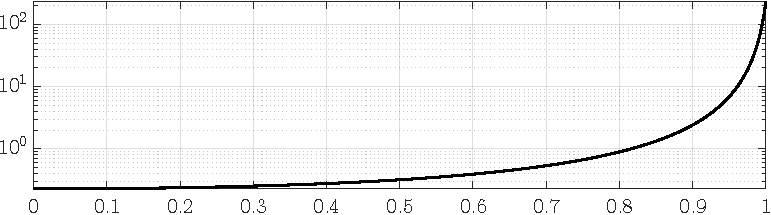
\includegraphics[width=0.7\columnwidth]{cost-cntrl-2.pdf}
\caption{Long-run average cost $J_{\infty}^{\star}(\mathit{\Phi})$ for the rotary inverted pendulum under the proposed infinite-horizon LQR with $n_f=0$ for $\Sigma_{w}=4\cdot 10^{-6} I_4$. See [4—Fig. 13] for similar results, obtained with $\Sigma_{w}=2.5\cdot 10^{-9} I_4$.}
\end{center}
\end{figure}
\vspace*{-10pt}
\setcounter{figure}{3}
\begin{figure}[h!]
\begin{center}
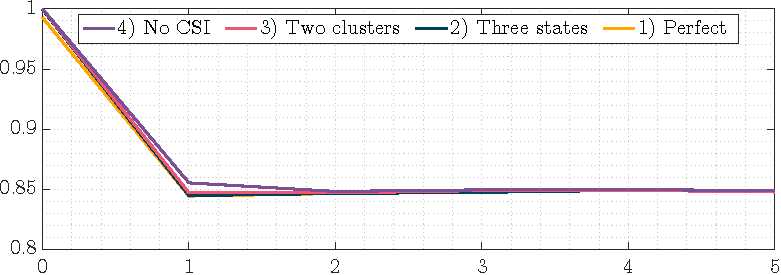
\includegraphics[width=0.7\columnwidth]{stability-cntrl-1.pdf}
\caption{The spectral radius of the mean-square stability verification matrix, $\rho(\mathit{\Lambda})$, as a function of the number of control inputs $n_f$ for the rotary inverted pendulum under the proposed infinite-horizon linear–quadratic regulation (LQR) with the dropout compensation factor $\mathit{\Phi}=I$}
\end{center}
\end{figure}
% \vspace*{10pt}
\begin{figure}[h!]
\begin{center}
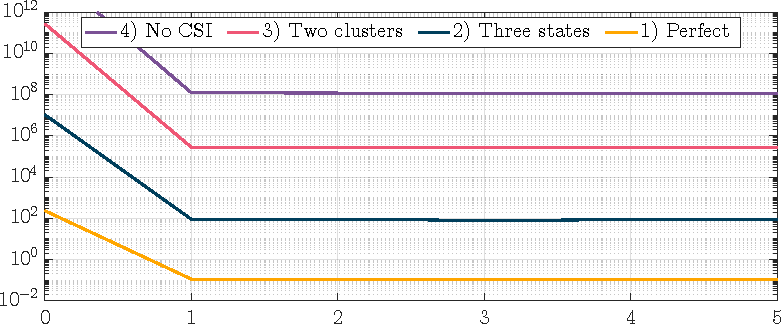
\includegraphics[width=0.7\columnwidth]{cost-cntrl-1.pdf}
\caption{The long-run average cost, $J_{\infty}^{\star}$, as a function of the number of control inputs $n_f$ for the rotary inverted pendulum under the proposed infinite-horizon linear–quadratic regulation (LQR) with the dropout compensation factor $\mathit{\Phi}=I$}
\end{center}
\end{figure}
% \vspace*{10pt}
\begin{figure}[h!]
\begin{center}
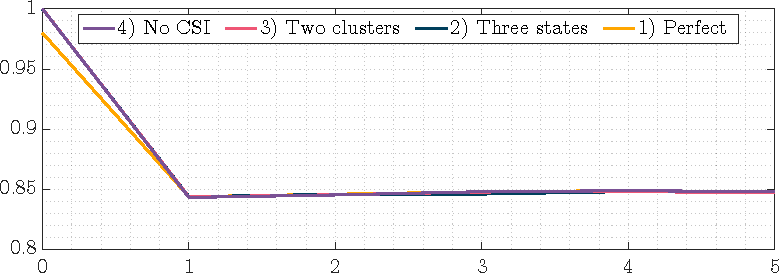
\includegraphics[width=0.76\columnwidth]{stability-cntrl-9.pdf}
\caption{The spectral radius of the mean-square stability verification matrix, $\rho(\mathit{\Lambda})$, as a function of the number of control inputs $n_f$ for the rotary inverted pendulum under the proposed infinite-horizon linear–quadratic regulation (LQR) with the dropout compensation factor $\mathit{\Phi}=0.921$}
\end{center}
\end{figure}
\vspace*{10pt}
\begin{figure}[h!]
\begin{center}
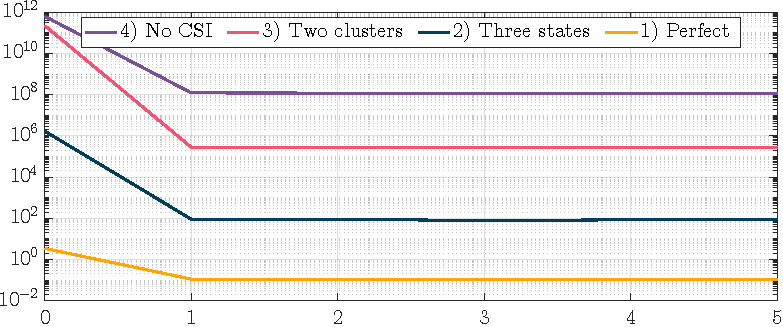
\includegraphics[width=0.76\columnwidth]{cost-cntrl-9.pdf}
\caption{The long-run average cost, $J_{\infty}^{\star}$, as a function of the number of control inputs $n_f$ for the rotary inverted pendulum under the proposed infinite-horizon linear–quadratic regulation (LQR) with the dropout compensation factor $\mathit{\Phi}=0.921$}
\end{center}
\end{figure}\\
\newpage
\begin{figure}[h!]
\begin{center}
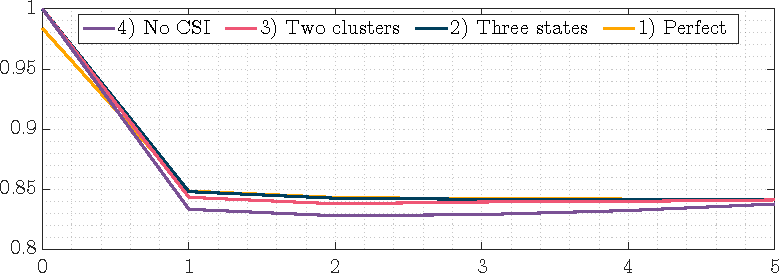
\includegraphics[width=0.76\columnwidth]{stability-cntrl-0.pdf}
\caption{The spectral radius of the mean-square stability verification matrix, $\rho(\mathit{\Lambda})$, as a function of the number of control inputs $n_f$ for the rotary inverted pendulum under the proposed infinite-horizon linear–quadratic regulation (LQR) with the dropout compensation factor $\mathit{\Phi}=0$}
\end{center}
\end{figure}
\begin{figure}[h!]
\begin{center}
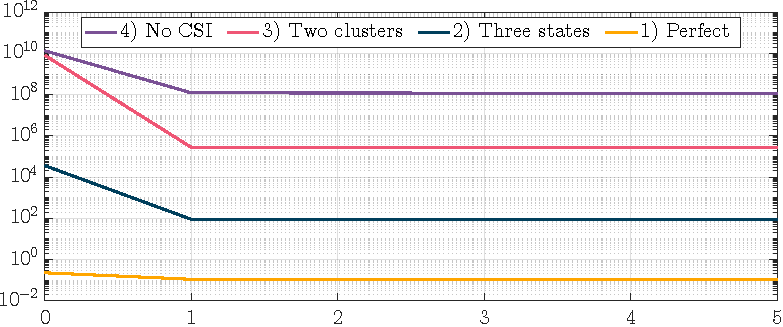
\includegraphics[width=0.76\columnwidth]{cost-cntrl-0.pdf}
\caption{The long-run average cost, $J_{\infty}^{\star}$, as a function of the number of control inputs $n_f$ for the rotary inverted pendulum under the proposed infinite-horizon linear–quadratic regulation (LQR) with the dropout compensation factor $\mathit{\Phi}=0$}
\end{center}
\end{figure}
%%
% As discussed in our response to the Reviewer's third comment, the value of $\rho(\mathit{\Lambda})$ relates to the maximal exponential decay rate.
Please also refer to our response to Reviewer 10's sixth comment on technical accuracy, in which we analyzed the closed-loop system performance under exceptionally high average message dropout probabilities exceeding $21.4$\%, which further increases with the size of the control message due to the growing number of future control inputs.
For the mode-independent scenario (No CSI) with $\mathit{\Phi}=0.1$, transmitting more than three future control inputs may destabilize the closed-loop system due to high message error rate. However, these observations may not apply to different plants and FSMCs. The presented framework allows us to investigate the impact of any specific message dropout strategy $\mathit{\Phi}$ on the transient and steady-state behavior of any linear plant controlled through an FSMC with potentially imperfect CSI.}\\[4mm]
%%%
\textbf{Reviewer 16---Comment 7---}\textit{%
How might the approach adapt to input/state constraints or nonlinear systems?}\\[2mm]
\textbf{Authors' response to comment 7:} \textcolor{black}{We thank the Reviewer for an insightful question. Although we do not yet have a ready extension for constrained and nonlinear systems, we may try to adopt the ideas of \cite{KOTHARE19961361} to incorporate constraints and \cite{10273597} to address nonlinearities.}\\[4mm]
%%%
\textbf{Authors' concluding remark:} \textcolor{black}{We thank the Reviewer for the valuable comments and suggestions. We sincerely hope the above explanations have adequately addressed the Reviewer's concerns.}
\putbib
\end{bibunit}
\end{document}
